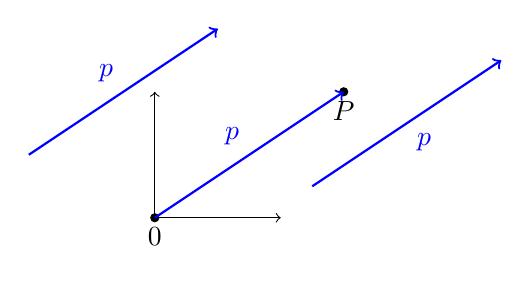
\begin{tikzpicture}[scale=0.8]
    \draw[<->](2,0,0)--(0,0,0)--(0,2,0);
    \draw[fill] (0,0) circle [radius=1.8pt] node[below]{$0$};
    \draw[fill] (3,2) circle [radius=1.8pt] node[below]{$P$};
    \draw[thick, blue, ->](-2,1) -- node[above left]{$\vect{p}$} +(3,2);
    \draw[thick, blue, ->](2.5,0.5) -- node[below right]{$\vect{p}$} +(3,2);
    \draw[thick, blue, ->](0,0) -- node[above left]{$\vect{p}$} +(3,2);
  \end{tikzpicture}
